\documentclass{article}
\usepackage{graphicx} % Required for inserting images
\usepackage{enumitem}
\usepackage{xcolor}
\usepackage{listings}
\usepackage{mathtools}
\usepackage{amsmath}
\newcommand{\logicarg}[2]{% \logicarg{<premise>}{<conclusion>}
  \begin{tabular}[t]{@{}l@{}}
    #1 \\ \hline #2
  \end{tabular}%
}

\setlength{\oddsidemargin}{-0.25in}
\setlength{\topmargin}{-0.5in}
\setlength{\headheight}{0cm}
\setlength{\headsep}{0cm}
\setlength{\textheight}{10in}
\setlength{\textwidth}{7in}
\setlength{\topskip}{0cm}

\begin{document}

\noindent\textbf{ComS 472 - PS10 \quad Due: Nov 24, 2024 \quad Name: Aren Ashlock}

\begin{enumerate}

% ------------------------------------- 1 DONE -------------------------------------

\item \textbf{(18 pts)} (Exercise 14.7) Let $H_x$ be a random variable denoting the handedness of an individual $x$, with possible values $l$ or $r$. A common hypothesis is that left- or right-handedness is inherited by a simple mechanism; that is, perhaps there is a gene $G_x$, also with values $l$ or $r$, and perhaps actual handedness turns out mostly the same (with some probability $s$) as the gene an individual possesses. Furthermore, perhaps the gene itself is equally likely to be inherited from either of an individual’s parents, with a small nonzero probability $m$ of a random mutation flipping the handedness.

\begin{center}
    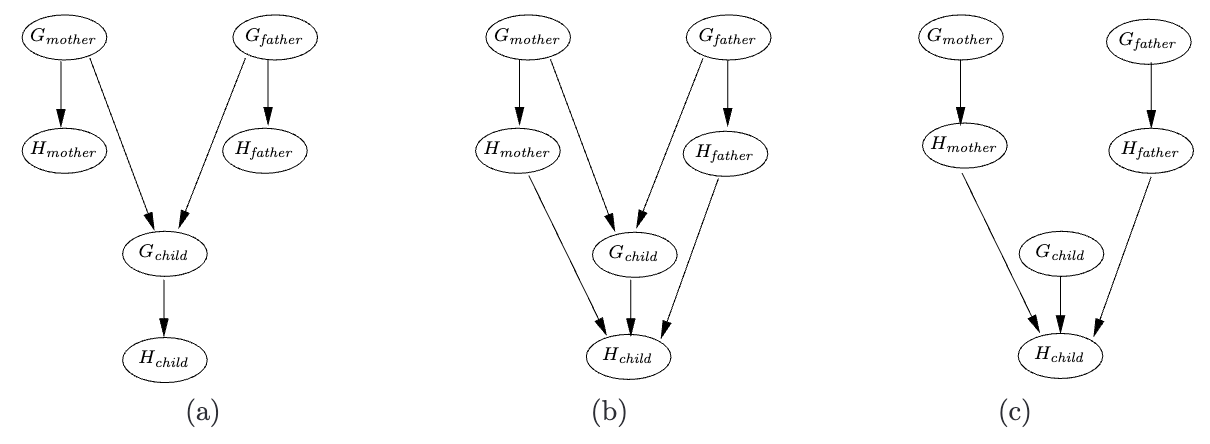
\includegraphics[scale=0.75]{472-PS10-Q1.png}
\end{center}

\begin{enumerate}[label=($\alph*$)]

    % ----------------------------------- 1a DONE -----------------------------------

    \item \textbf{(2 pts)} Which of the three networks in the above figure claim that

    \begin{equation*}
        \mathbf{P}(G_{father},G_{mother},G_{child})=\mathbf{P}(G_{father})\mathbf{P}(G_{mother})\mathbf{P}(G_{child})
    \end{equation*}

    \color{blue}
        \textbf{C}, all genes are independent of each other
    \color{black}

    % -------------------------------------------------------------------------------

    % ----------------------------------- 1b DONE -----------------------------------

    \item \textbf{(3 pts)} Which of the three networks make independence claims that are consistent with the hypothesis about the inheritance of handedness?

    \color{blue}
        \textbf{A and B}, the gene of the child is dependent on the parents, but the parents are independent, which both contain.
    \color{black}

    % -------------------------------------------------------------------------------

    % ----------------------------------- 1c DONE -----------------------------------

    \item \textbf{(3 pts)} Which of the three networks is the best description of the hypothesis?

    \color{blue}
        \textbf{A}, it's either A or B since the hypothesis notes a dependence of the child's gene on the parents' gene. But, the hypothesis doesn't mention anything about the handedness of the child depending on the handedness of the parents.
    \color{black}

    % -------------------------------------------------------------------------------

    % ----------------------------------- 1d DONE -----------------------------------

    \item \textbf{(4 pts)} Write down the CPT for the $G_{child}$ node in network (a), in terms of $s$ and $m$.

    \color{blue}
        \begin{tabular}{ |c c|c| } 
             \hline
             $G_{father}$ & $G_{mother}$ & $P(G_{child}=l|G_{father},G_{mother})$ \\
             \hline
             $l$ & $l$ & $1-m$ \\
             $l$ & $r$ & $0.5(1-m)+0.5(m)=0.5$ \\
             $r$ & $l$ & $0.5$ \\
             $r$ & $r$ & $m$ \\
             \hline
        \end{tabular}
    \color{black}

    % -------------------------------------------------------------------------------

    % ----------------------------------- 1e DONE -----------------------------------

    \item \textbf{(6 pts)} Suppose that $P(G_{father} = l) = P(G_{mother} = l) = q$. In network (a), derive an expression for $P(G_{child} = l)$ in terms of $m$ and $q$ only, by conditioning on its parent nodes.


    \color{blue}
        $P(G_{child} = l) = \sum P(G_{child} = l | G_{father} \wedge G_{mother})P(G_{father})P(G_{mother})$\\
        $P(G_{child} = l) = (1-m)(q^2) + 2\times(0.5)(q)(1-q) + (m)(1-q)^2$\\
        $P(G_{child} = l) = q^2 - mq^2 + q - q^2 + m - 2mq + mq^2$\\
        $P(G_{child} = l) = q + m - 2mq$
    \color{black}

    % -------------------------------------------------------------------------------
    
    \end{enumerate}

% ----------------------------------------------------------------------------------

% ------------------------------------- 2 DONE -------------------------------------

\item \textbf{(10 pts)} (Exercise 14.13)  In your local nuclear power station, there is an alarm that senses when a temperature gauge exceeds a given threshold. The gauge measures the temperature of the core. Consider the Boolean variables $A$ (alarm sounds), $F_A$ (alarm is faulty), and $F_G$ (gauge is faulty) and the multivalued nodes $G$ (gauge reading) and $T$ (actual core temperature).

\begin{enumerate}[label=($\alph*$)]

    % ----------------------------------- 2a DONE -----------------------------------

    \item \textbf{(6 pts)} Draw a Bayesian network for this domain, given that the gauge is more likely to fail when the core temperature gets too high.

    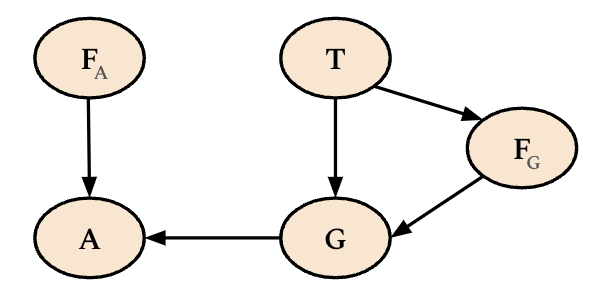
\includegraphics[scale=0.5]{472-PS10-Q2A.png}

    % -------------------------------------------------------------------------------

    % ----------------------------------- 2c DONE -----------------------------------

    \addtocounter{enumii}{1} \item \textbf{(4 pts)} Suppose there are just two possible actual and measured temperatures, normal and high; the probability that the gauge gives the correct temperature is $x$ when it is working, but $y$ when it is faulty. Give the conditional probability table associated with $G$.

    \color{blue}
        \begin{tabular}{ |c c|c| } 
             \hline
             $T$ & $F_G$ & $P(G=normal|T, F_G)$ \\
             \hline
             $normal$ & $f$ & $x$ \\
             $normal$ & $t$ & $y$ \\
             $high$ & $f$ & $1-x$ \\
             $high$ & $t$ & $1-y$ \\
             \hline
        \end{tabular}
    \color{black}

    % -------------------------------------------------------------------------------
    
    \end{enumerate}

% ----------------------------------------------------------------------------------

% ------------------------------------- 3 DONE -------------------------------------

\item \textbf{(12 pts)} (Exercise 14.16) Consider the Bayes net shown below.

\begin{center}
    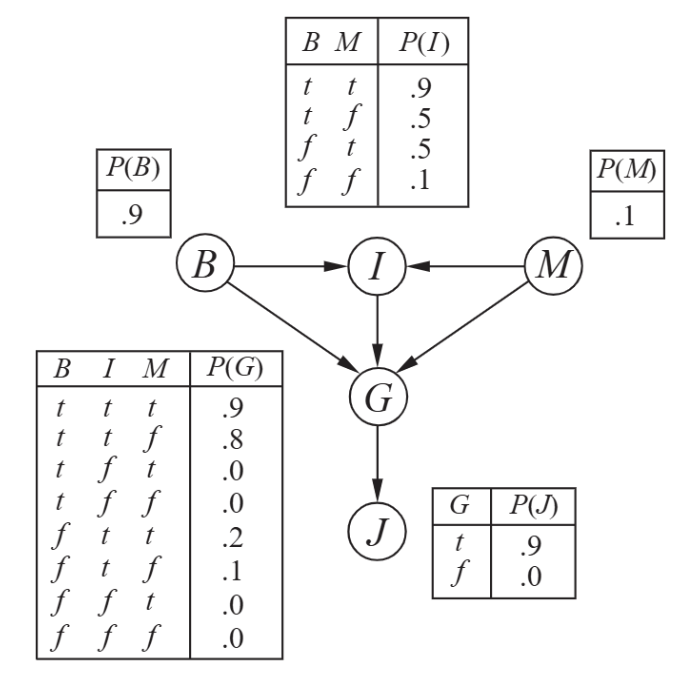
\includegraphics[scale=0.75]{472-PS10-Q3.png}
\end{center}

    \begin{enumerate}[label=($\alph*$)]

    % ----------------------------------- 3a DONE -----------------------------------

    \item \textbf{(3 pts)} Which of the following are asserted by the network structure?

    \begin{equation}
        \mathbf{P}(B,I,M)=\mathbf{P}(B)\mathbf{P}(I)\mathbf{P}(M)
    \end{equation}
    \begin{equation}
        \mathbf{P}(J|G)=\mathbf{P}(J|G,I)
    \end{equation}
    \begin{equation}
        \mathbf{P}(M|G,B,I)=\mathbf{P}(M|G,B,I,J)
    \end{equation}

    \color{blue}
        \textbf{2} (conditional independence, $I$ is not in $MB(J)$ so $I$ has no impact)\\
        \textbf{and 3} (conditional independence, $J$ is not in $MB(M)$ so $J$ has no impact)
    \color{black}

    % -------------------------------------------------------------------------------

    % ----------------------------------- 3b DONE -----------------------------------

    \item \textbf{(3 pts)} Calculate the probability $P(b, i, \neg m, g, j)$.

    \color{blue}
        $P(b, i, \neg m, g, j) = P(b)P(\neg m)P(i | b \wedge \neg m)P(g | b \wedge \neg m \wedge i)P(j | g)$\\
        $P(b, i, \neg m, g, j) = 0.9 * (1 - 0.1) * 0.5 * 0.8 * 0.9$\\
        \textbf{Answer:} $P(b, i, \neg m, g, j) = 0.2916$
    \color{black}

    % -------------------------------------------------------------------------------

    % ----------------------------------- 3c DONE -----------------------------------

    \item \textbf{(6 pts)} Calculate the probability that someone goes to jail given that they broke the law, have been indicted, and face a politically motivated prosecutor.

    \color{blue}
        $P(j|b \wedge i \wedge m) = \sum P(j|G)P(G|b \wedge i \wedge m)$\\
        $P(j|b \wedge i \wedge m) = P(j|g)P(g|b \wedge i \wedge m) + P(j|\neg g)P(\neg g|b \wedge i \wedge m)$\\
        $P(j|b \wedge i \wedge m) = 0.9(0.9) + 0.0(1-0.9)$\\
        \textbf{Answer:} $P(j|b \wedge i \wedge m) = 0.81$
    \color{black}

    % -------------------------------------------------------------------------------
    
    \end{enumerate}

% ----------------------------------------------------------------------------------

% ------------------------------------- 4 DONE -------------------------------------

\item \textbf{(10 pts)} (Exercise 14.18(a)) Consider the variable elimination algorithm given below. For the shown burglary-alarm network, applies variable elimination to the query

\begin{equation*}
    \mathbf{P}(Burglary|JohnCalls=True,MaryCalls=True).
\end{equation*}

Perform the calculations indicated and check that the answer is correct.

\begin{center}
    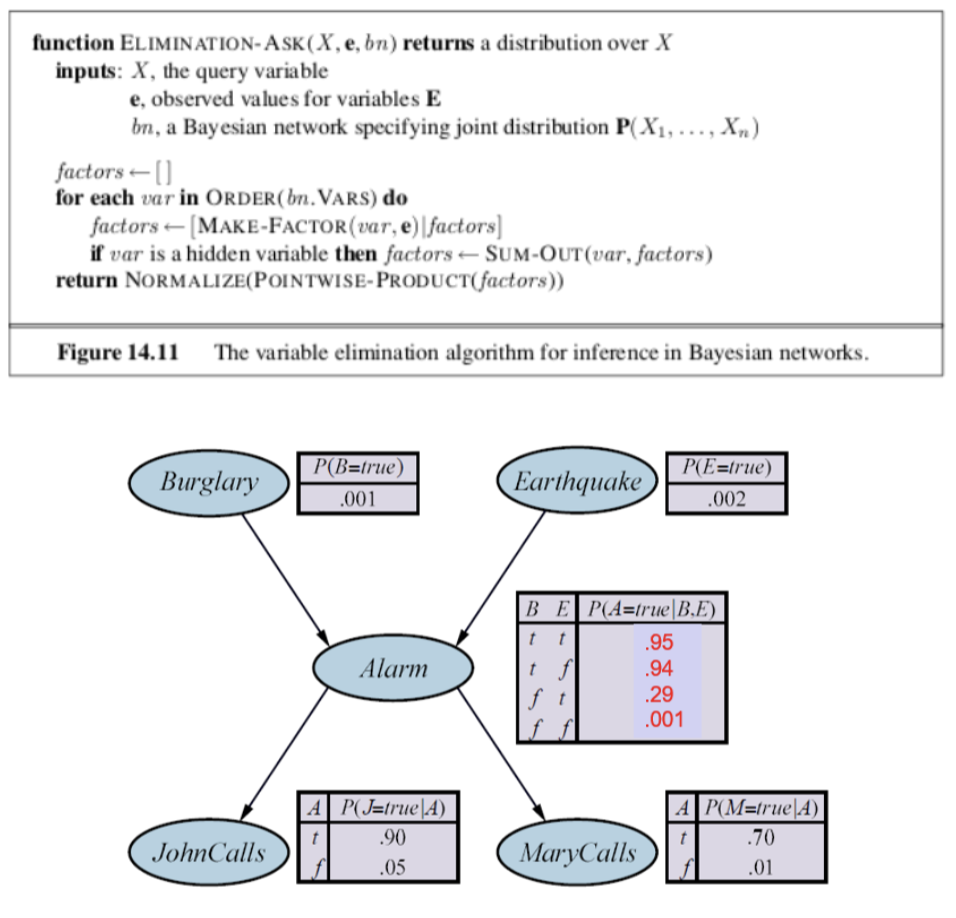
\includegraphics[scale=0.6]{472-PS10-Q4.png}
\end{center}

\color{blue}
    $\alpha P(B) \sum_{e'} P(e') \sum_{a'} P(a'|B, e')P(j|a')P(m|a')$\\
    $\alpha P(B) \sum_{e'} P(e') (\begin{pmatrix}0.95&0.94&0.29&0.001\end{pmatrix}*0.90*0.70+\begin{pmatrix}0.05&0.06&0.71&0.999\end{pmatrix}*0.05*0.01)$\\
    $\alpha P(B) \sum_{e'} P(e') (\begin{pmatrix}0.5985&0.5922&0.1827&0.00063\end{pmatrix}+\begin{pmatrix}0.000025&0.00003&0.000355&0.0004995\end{pmatrix})$\\
    $\alpha P(B) \sum_{e'} P(e') \begin{pmatrix}0.598525&0.59223&0.183055&0.0011295\end{pmatrix}$\\
    $\alpha P(B) (0.002 * \begin{pmatrix}0.598525&0.183055\end{pmatrix} + 0.998 * \begin{pmatrix}0.59223&0.0011295\end{pmatrix})$\\
    $\alpha P(B) (\begin{pmatrix}0.00119705&0.00036611\end{pmatrix} + \begin{pmatrix}0.59104554&0.001127251\end{pmatrix})$\\
    $\alpha P(B) \begin{pmatrix}0.59224259&0.001493351\end{pmatrix}$\\
    $\alpha \begin{pmatrix}0.001&0.999\end{pmatrix} \begin{pmatrix}0.59224259&0.001493351\end{pmatrix}$\\
    $\alpha \begin{pmatrix}0.00059224259&0.00149185765\end{pmatrix}$\\
    $\approx \langle0.284,0.716\rangle$, \textbf{which is correct}
\color{black}

% ----------------------------------------------------------------------------------

\end{enumerate}
\end{document}